
\documentclass[10pt]{beamer}

\usetheme{Frankfurt}
\usecolortheme{beaver}
\setbeamertemplate{footline}[frame number]

\AtBeginSection[]{
  \begin{frame}
  \vfill
  \centering
  \begin{beamercolorbox}[sep=8pt,center,shadow=true,rounded=true]{title}
    \usebeamerfont{title}\insertsectionhead\par%
  \end{beamercolorbox}
  \vfill
  \end{frame}
}

\usepackage[french]{babel}
\usepackage[utf8]{inputenc}
\usepackage{graphicx}
\usepackage{caption} 
\usepackage{xcolor} 
\usepackage{amsmath}

\newcommand{\source}[1]{\caption*{\centering\small Source: #1}}
\usepackage[font=small, labelfont=bf]{caption}

\title[Dynamique cardiaque]{Cycles limites et boucles de propagation dans la dynamique électrique du cœur}
\author{El Yousfi Alaoui Nabil}
\date{2025/2026}


\begin{document}

\begin{frame}
\titlepage 
\end{frame}


\begin{frame}
\frametitle{Plan de l'exposé} 
\tableofcontents 
\end{frame}

\section{Introduction et motivation}

\begin{frame}
\frametitle{Introduction}
\framesubtitle{Les ondes spirales cardiaques}
%\begin{columns}
%\column{0.55\textwidth}
%\begin{small}
%\begin{itemize}
%  \item Les arythmies cardiaques, comme la tachycardie ventriculaire et la fibrillation, sont des troubles du rythme qui peuvent entraîner une mort subite en quelques minutes.
%  \item Dans de nombreux cas, ces arythmies sont entretenues par une onde électrique auto‑entretenue qui tourne dans le muscle cardiaque : une onde spirale.
%  \item Modéliser ce phénomène permet d’en comprendre les mécanismes profonds et d’envisager des stratégies thérapeutiques pour interrompre ces ondes, par exemple par défibrillation électrique.
%\end{itemize}
%\end{small}

%\column{0.45\textwidth}
\centering
\begin{figure}
\caption{Onde spirale simulée dans un tissu cardiaque virtuel}
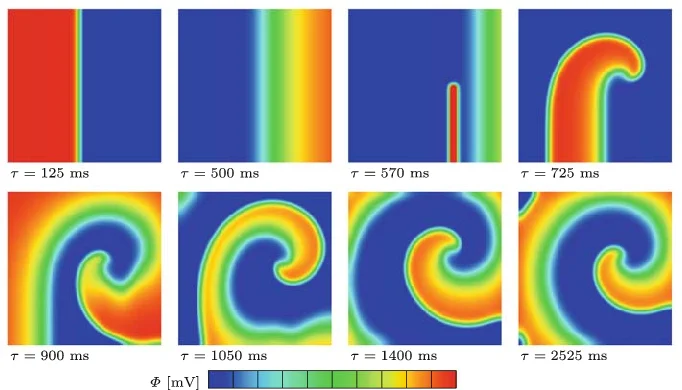
\includegraphics[scale = 0.32]{Figures/onde_spirale_intro.png}
\source{Atrial and ventricular fibrillation: Computational simulation of spiral waves in cardiac tissue}
\end{figure}
%\end{columns}
\end{frame}
\section{Contexte biologique et naissance du modèle}


%Diapo 1
\begin{frame}
\frametitle{Contexte biologique et naissance du modèle}
\framesubtitle{Polarisation, dépolarisation et canaux ioniques}

\begin{columns}
\column{0.5\textwidth}
\begin{small}
\begin{itemize}
  \item \textbf{Au repos} : l'intérieur de la cellule est négatif ($\approx -70$ mV) par rapport à l'extérieur : c'est la \alert{polarisation}.
  \item Maintien par la pompe Na$^+$/K$^+$ et des canaux de fuite.
  \item \textbf{Dépolarisation} : ouverture de canaux Na$^+$ voltage‑dépendants $\rightarrow$ entrée de Na$^+$ $\rightarrow$ le potentiel devient positif.
  \item \textbf{Repolarisation} : inactivation des canaux Na$^+$, ouverture de canaux K$^+$ $\rightarrow$ sortie de K$^+$ $\rightarrow$ retour au repos.
\end{itemize}
\end{small}
\column{0.5\textwidth}
\begin{figure}[t]
    \centering
    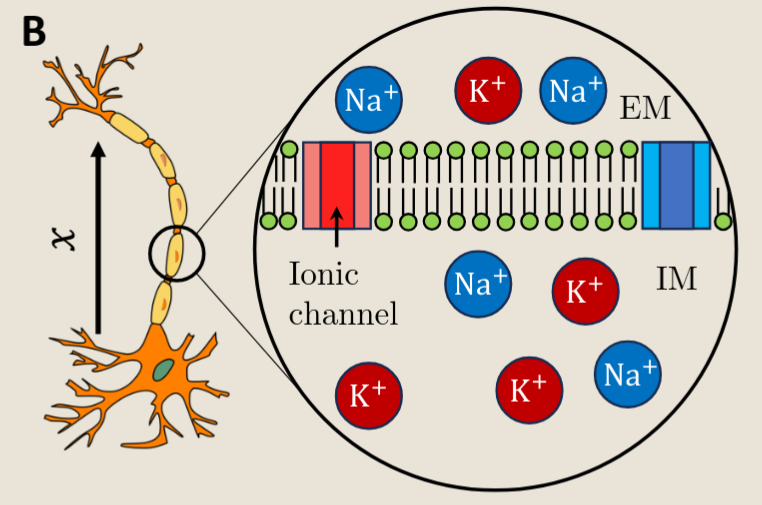
\includegraphics[width=\linewidth]{Figures/canaux_ioniques.png}
    \caption{Canaux ioniques}
    %\source{Six decades of the FitzHugh-Nagumo model: A guide through its spatio-
%temporal dynamics and influence across disciplines}
\end{figure}
\end{columns}
\end{frame}

%Diapo 2
\begin{frame}
\frametitle{Contexte biologique et naissance du modèle}
\framesubtitle{L'excitabilité des cellules cardiaques}
\begin{columns}
\column{0.6\textwidth}
\begin{itemize}
  \item Les cellules du muscle cardiaque (cardiomyocytes) sont \alert{excitables}.
  \item Un stimulus suffisant déclenche un \textbf{potentiel d'action} : 
    dépolarisation rapide suivie d'une repolarisation.
  \item Ce signal électrique se propage de proche en proche et coordonne la contraction.
\end{itemize}
\column{0.4\textwidth}

\begin{figure}
    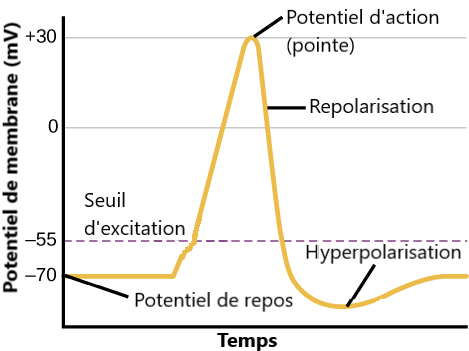
\includegraphics[width=\linewidth]{Figures/potentiel_action.png}
    \caption{Potentiel d'action} \label{Figure-1}
    %\source{ Image modifiée à partir de "How neurons communicate: Figure 3," par OpenStax College, Biology (CC BY 3.0).}
\end{figure}
\end{columns}
\end{frame}

%Diapo 3
\begin{frame}
\frametitle{Contexte biologique et naissance du modèle}
\framesubtitle{Modèle de Hodgkin-Huxley (1952) – Circuit équivalent}
\centering
\begin{figure}
  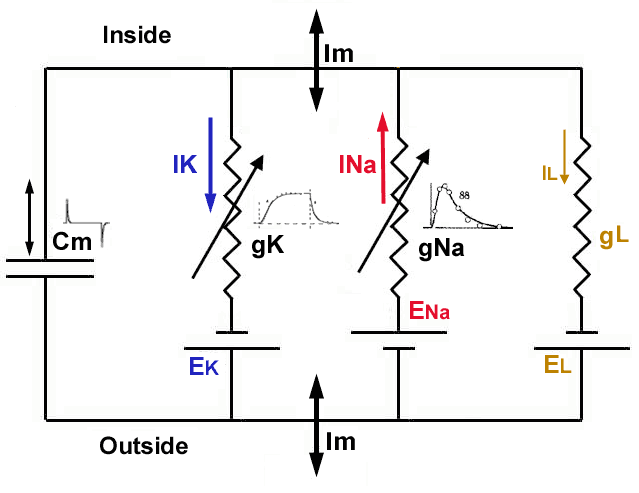
\includegraphics[scale = 0.35]{Figures/HH.png} 
  \caption{Circuit équivalent : 4 branches parallèles (Na\(^+\), K\(^+\), fuite, capacité).}
  %\source{University of Pennsylvania School of Arts and Sciences. (n.d.). Circuit diagram and related equation. SAS Lab Manuals.}
\vspace{0.3cm}
\end{figure}
\end{frame}



%Diapo 4
\begin{frame}
\frametitle{Contexte biologique et naissance du modèle}
\framesubtitle{Modèle de Hodgkin-Huxley (1952) – description mathématique}
%\column{0.6\textwidth}
\textbf{Équation de la membrane :}
\[
C_m\frac{dV}{dt} = -\underbrace{\bar{g}_{\text{Na}} m^3 h (V-E_{\text{Na}})}_{\text{courant Na\(^+\)}}
                 -\underbrace{\bar{g}_{\text{K}} n^4 (V-E_{\text{K}})}_{\text{courant K\(^+\)}}
                 -\underbrace{g_{\text{L}}(V-E_{\text{L}})}_{\text{fuite}}
                 + I_{\text{app}}
\]
\textbf{Équations des portes (gating) :}
\[
\frac{dm}{dt} = \alpha_m(V)(1-m) - \beta_m(V)m \quad \text{(activation Na\(^+\))}
\]
\[
\frac{dh}{dt} = \alpha_h(V)(1-h) - \beta_h(V)h \quad \text{(inactivation Na\(^+\))}
\]
\[
\frac{dn}{dt} = \alpha_n(V)(1-n) - \beta_n(V)n \quad \text{(activation K\(^+\))}
\]
\end{frame}


%Diapo 5
%\begin{frame}
%\frametitle{Contexte biologique et naissance du modèle}
%\framesubtitle{Difficultés du modèle Hodgkin‑Huxley}
%\begin{itemize}
%  \item \textbf{Système à 4 variables} : $V$, $m$, $h$, $n$ $\Rightarrow$ espace des phases de dimension 4.
%  \item \textbf{Non‑linéarités complexes} : les taux $\alpha(V)$, $\beta(V)$ et les produits de puissances ($m^3h$, $n^4$).
%  \item \textbf{Absence d’outils géométriques simples} :
%  \begin{itemize}
%    \item Pas de portrait de phase en 2D.
%    \item Pas d’isoclines visuellement exploitables.
%  \end{itemize}
%  \item \textbf{Impossible d’obtenir des formules analytiques} pour :
%  \begin{itemize}
%    \item le seuil d’excitation,
%    \item la fréquence des oscillations,
%    \item les conditions de bifurcation.
%  \end{itemize}
%  \item \textbf{Coût de simulation prohibitif} pour de grands réseaux :
%  \begin{itemize}
%    \item Un tissu cardiaque $\approx 10^6$ cellules $\times$ 4 EDOs $\Rightarrow$ millions d’équations.
%  \end{itemize}
%\end{itemize}
%\end{frame}

%Diapo 6
\begin{frame}
\frametitle{Contexte biologique et naissance du modèle}
\framesubtitle{La réduction de FitzHugh‑Nagumo (1961)}
\alert{\textbf{En exploitant les échelles de temps}}
\begin{itemize}
  \item Dans HH, la porte d’activation sodium $m$ est \textbf{très rapide} : $m \approx m_\infty(V)$ (instantanée).
  \item Les variables $h$ (inactivation Na$^+$) et $n$ (activation K$^+$) évoluent \textbf{lentement} et sont \textbf{corrélées}.
  \item On les remplace par une seule variable lente $w$ (récupération).
\end{itemize}

\alert{\textbf{Le modèle à 2 variables}}
\[
\begin{cases}
  \displaystyle \frac{dv}{dt} = v - \frac{v^3}{3} - w + I_{\text{app}} \\[8pt]
  \displaystyle \frac{dw}{dt} = \varepsilon (v + a - b w)
\end{cases}
\]
\begin{itemize}
  \item $v$ : variable rapide (potentiel de membrane).
  \item $w$ : variable lente (recouvrement).
  \item $\varepsilon \ll 1$ : petit paramètre garantissant la séparation d’échelles.
  \item $a$, $b$, $I_{\text{app}}$ : paramètres de contrôle du comportement.
\end{itemize}
\end{frame}
\section{Analyse mathématique du système FHN}


%Diapo 1
\begin{frame}
\frametitle{Analyse mathématique du système FHN}
\framesubtitle{Système de FitzHugh-Nagumo : écriture et isoclines}
\begin{columns}
\column{0.5\textwidth}
\alert{\textbf{Le modèle à deux variables}}
\[
\begin{cases}
  \displaystyle \frac{dv}{dt} = v - \frac{v^3}{3} - w + I_{\text{app}} \\[8pt]
  \displaystyle \frac{dw}{dt} = \varepsilon (v + a - b w)
\end{cases}
\]
\alert{\textbf{Isoclines (nullclines)}}
\begin{itemize}
  \item $\dfrac{dv}{dt}=0 \; \implies ; w = v - \dfrac{v^3}{3} + I_{\text{app}}$ \hfill (cubique)
  \item $\dfrac{dw}{dt}=0 \; \implies ; w = \dfrac{v+a}{b}$ \hfill (droite)
\end{itemize}

\column{0.5\textwidth}
\centering
\begin{figure}
  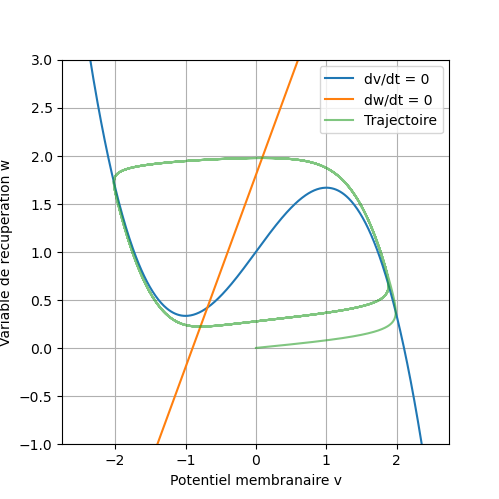
\includegraphics[width=\linewidth]{Figures/FHN.png}
  \caption{Portrait de phase du modèle de FitzHugh-Nagumo}
  %\source{ FitzHugh-Nagumo model, Scholarpedia, modifié d'après FitzHugh 1961}
\end{figure}
\end{columns}
\vspace{0.2cm}
\centerline{L’intersection des isoclines nulles donne le(s) point(s) fixe(s) du système.}
\end{frame}

%Diapo 2
\begin{frame}
\frametitle{Analyse mathématique du système FHN}
\framesubtitle{Point(s) fixe(s) et stabilité linéaire}
\begin{itemize}
  \item \alert{Point(s) fixe(s) :} intersection des deux isoclines nulles.
  \[
  \begin{cases}
    w^* = v^* - \dfrac{v^{*3}}{3} + I_{\text{app}} \\[6pt]
    w^* = \dfrac{v^*+a}{b}
  \end{cases}
  \]
  \item Suivant $I_{\text{app}}$ (ou $a$), on obtient 1 ou 3 points fixes.
  \item On se place ici dans le cas usuel d’un point fixe unique.
\end{itemize}

\alert{Linéarisation autour du point fixe $(v^*,w^*)$}
\[
\mathbf{J} = \begin{pmatrix}
  1 - v^{*2} & -1 \\
  \varepsilon & -\varepsilon b
\end{pmatrix}
\]
\begin{itemize}
  \item Trace : $\operatorname{tr}(\mathbf{J}) = 1 - v^{*2} - \varepsilon b$
  \item Déterminant : $\det(\mathbf{J}) = \varepsilon\bigl[1 + b(v^{*2}-1)\bigr]$
\end{itemize}
\end{frame}

%Diapo 3
\begin{frame}
\frametitle{Analyse mathématique du système FHN}
\framesubtitle{Stabilité et nature du point fixe}

\alert{\textbf{Conditions de stabilité (Routh-Hurwitz en 2D)}}
\begin{itemize}
  \item Un point fixe est \textbf{asymptotiquement stable} ssi 
  \(\operatorname{tr}(\mathbf{J}) < 0\) \textbf{et} \(\det(\mathbf{J}) > 0\).
  \item Ici, \(\det(\mathbf{J}) > 0\) pour les paramètres biologiques usuels (pas de point selle).
  \item La stabilité est donc gouvernée par le \textbf{signe de la trace}.
\end{itemize}

\alert{\textbf{Valeurs propres et classification}}
\[
\lambda_{\pm} = \frac{\operatorname{tr}(\mathbf{J}) \pm \sqrt{\Delta}}{2}, \quad
\Delta = \operatorname{tr}(\mathbf{J})^2 - 4\det(\mathbf{J})
\]
\begin{itemize}
  \item \(\operatorname{tr} < 0\) et \(\Delta > 0\) : \textbf{nœud stable} (amortissement monotone).
  \item \(\operatorname{tr} < 0\) et \(\Delta < 0\) : \textbf{foyer stable} (oscillations amorties).
  \item \(\operatorname{tr} > 0\) : \textbf{instable} (nœud ou foyer).  
  \item La frontière \(\operatorname{tr} = 0\) correspond à des valeurs propres imaginaires pures \(\Rightarrow\) \textbf{bifurcation de Hopf}.
\end{itemize}
\end{frame}


%Diapo 4
\begin{frame}
\frametitle{Analyse mathématique du système FHN}
\framesubtitle{Bifurcation de Hopf et naissance d’un cycle limite}
\alert{\textbf{Paramètre de bifurcation}} : $I_{\text{app}}$ ou $a$, ou $b$

Lorsque $I_{\text{app}}$ varie, le point fixe se déplace le long de la cubique.
\[
1 - v^{*2} = \varepsilon b \quad \text{(trace nulle)} \;\Longrightarrow\; \text{Bifurcation de Hopf.}
\]

\begin{itemize}
  \item Si $v^*$ est sur une \textbf{branche extérieure} ($|v^*|$ grand) : trace $<0$ $\rightarrow$ point fixe stable.
  \item Si $v^*$ est sur la \textbf{branche médiane} ($|v^*|$ petit, pente $>1$) : trace $>0$ $\rightarrow$ point fixe instable.
\end{itemize}

\alert{\textbf{Condition pour un cycle limite}}
\[
\varepsilon b < 1 \quad\text{(condition faible pour $\varepsilon$ petit)}
\]
Quand le point fixe devient instable, les trajectoires sont confinées par la cubique $\rightarrow$ un \textbf{cycle limite stable} apparaît (oscillations auto-entretenues).
\end{frame}
\section{Modèle électronique}

%diapo 1
\begin{frame}
\frametitle{Modèle électronique}
\framesubtitle{Pourquoi une réalisation analogique ?}
\begin{itemize}
  \item \alert{Objectif :} observer physiquement les oscillations (cycle limite) du FHN.
  \item \alert{Problème :} la cubique \(v - \frac{v^3}{3}\) n’est pas directement réalisable avec des composants simples.
  \item \alert{Solution :} remplacer la cubique par une approximation linéaire par morceaux à 3 segments.
\end{itemize}
\vspace{0.3cm}
\alert{\textbf{Principe de l’approximation}}
\begin{itemize}
  \item On utilise une fonction affine par morceaux \(f(v)\) qui reproduit :
  \begin{itemize}
    \item une pente négative pour \(|v|\) petit 
    \item des pentes positives pour \(|v|\) grand 
  \end{itemize}
  \item Le circuit électronique est réalisable par des amplificateurs opérationnels.
\end{itemize}
\vspace{0.3cm}
\end{frame}

%Diapo2
\begin{frame}
\frametitle{Modèle électronique}
\framesubtitle{Principe du générateur de courant non linéaire}

\begin{block}{Rôle de la saturation}
La saturation de l'amplificateur opérationnel crée deux ruptures de pente dans la caractéristique \(I(V_2)\), permettant d'obtenir une approximation linéaire par morceaux de la non-linéarité cubique du modèle de FitzHugh--Nagumo.
\end{block}
\vspace{0.1cm}
\begin{columns}[T]
\column{0.5\textwidth}
\small
\[
h(V_{2})=
\begin{cases}
V_{+}
& \text{si } V_{2}>V_* \\[6pt]
\left(1+\dfrac{R_1}{R_2}\right)V_{2}
& \text{si } -V_*<V_{2}<V_* \\[6pt]
V_{-}
& \text{si } V_{2}< -V_*
\end{cases}
\]
\[
\text{où : }  V_*=\dfrac{R_2}{R_1+R_2}\,V_{\mathrm{sat}}
\]
\[
\text{on a alors : } I=\frac{V_2-h(V_2)}{R_3} = -f(V_{2}) 
\]
\column{0.5\textwidth}
\centering
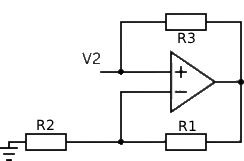
\includegraphics[width=\linewidth]{Figures/circuit.png}
\end{columns}
\end{frame}

%Diapo3
\begin{frame}
\frametitle{Modèle électronique}
\framesubtitle{Approximation linéaire par morceaux de la cubique}
\centering
\begin{figure}
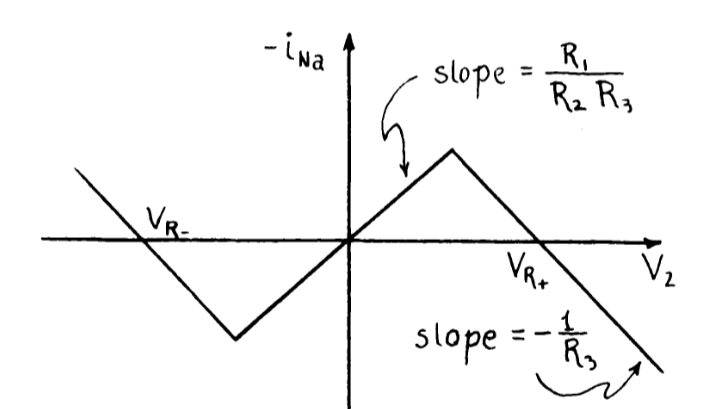
\includegraphics[scale = 0.4]{Figures/Linear_response.png}
\caption{Modèle linéaire}
%\source{James P.Keener, Analog Circuitry for the van der Pol and FitzHugh-Nagumo Equations}
\end{figure}
\vspace{0.3cm}
\end{frame}

%diapo4
\begin{frame}
\frametitle{Modèle électronique}
\framesubtitle{Inductance simulée par circuit à résistance négative}

\begin{block}{Rôle de l'inductance simulée}
L'association des composants passifs et de l'amplificateur opérationnel permet de synthétiser un comportement inductif sans utiliser de bobine réelle. 
\end{block}

\begin{columns}[T]
\column{0.5\textwidth}
\vspace{1.2cm}
\begin{equation}
\boxed{
C_2 R_5 R_4 \frac{di_2}{dt} + R_5\, i_2 = v - v_0
}
\end{equation}
%\[
%C_1 \frac{dv}{dt} = i_0 - f(v) - i_2\left(1 - \frac{R_5}{R_4}\right) - \frac{v - v_0}{R_4}
%\]

\centering

\column{0.5\textwidth}
\centering
\begin{figure}
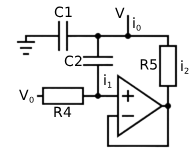
\includegraphics[scale = 0.6]{Figures/circuit1.png}
\caption{Schéma du montage à inductance simulée}
\end{figure}
\end{columns}


\end{frame}

%diapo5
\begin{frame}
\frametitle{Modèle électronique}
\framesubtitle{Circuit complet et équations du système}

\begin{block}{Circuit complet}
On monte un montage suiveur à un potentiomètre pour régler la tension d'entrée \(v_0\), 
suivi par l'inducteur simulé, et enfin le générateur de courant non linéaire réalisant la caractéristique \(f(v)\).
\end{block}

\vspace{0.1cm}

\begin{columns}[T]
\column{0.5\textwidth}
\small
\begin{equation}
\boxed{C_2 R_4 R_5 \frac{di_2}{dt} + R_5 i_2 = v - v_0}
\end{equation}
\nonumber
\vspace{0.3cm}
\begin{equation}
\boxed{C_1 \frac{dv}{dt} = i_0 - f(v) - i_2\left(1 - \frac{R_5}{R_4}\right) - \frac{v - v_0}{R_4}}
\end{equation}
\vspace{0.2cm}
\centering
\textit{(Équations du système analogue à FHN)}

\column{0.5\textwidth}
\centering
\begin{figure}
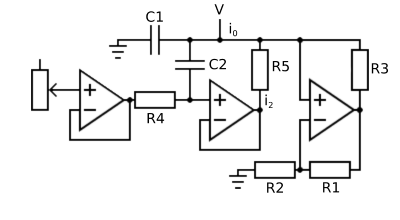
\includegraphics[width=\linewidth]{Figures/circuit_complet.png}
\caption{Schéma complet du modèle}
\end{figure}
\end{columns}
\end{frame}

\begin{frame}
\frametitle{Modèle électronique}
\framesubtitle{Allure prédite pour un modèle linéaire}

\begin{figure}
  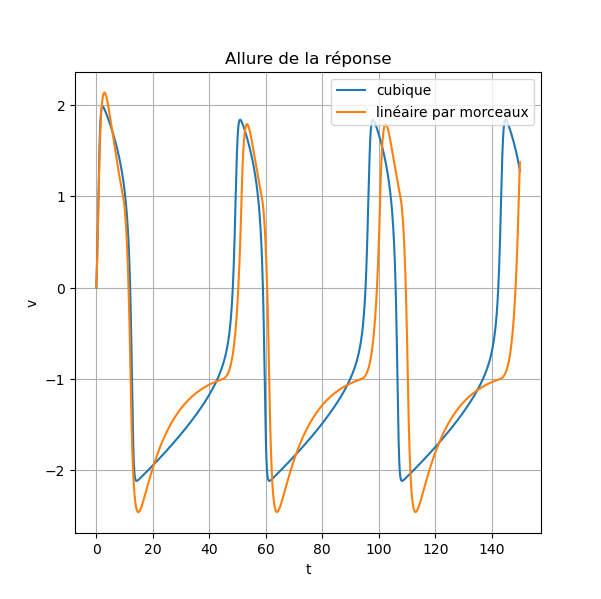
\includegraphics[scale = 1]{Figures/Linéaire.png}
  \caption{comparaison entre modèle linéaire par morceaux et modèle avec cubique}



\section{Simulation numérique du modèle diffusif FHN}

\begin{frame}
\frametitle{Simulation numérique}
\framesubtitle{Équation de réaction‑diffusion de FitzHugh‑Nagumo}
\begin{itemize}
  \item Pour modéliser un tissu cardiaque, on étend le système à un domaine spatial : chaque point est un oscillateur FHN couplé aux voisins par diffusion.
  \item Le modèle devient une équation de réaction‑diffusion :
  \[
  \begin{cases}
    \displaystyle \frac{\partial v}{\partial t} = D \nabla^2 v + v - \frac{v^3}{3} - w + I_{\text{app}} \\[8pt]
    \displaystyle \frac{\partial w}{\partial t} = \varepsilon (v + a - b w)
  \end{cases}
  \]
  où $D$ est le coefficient de diffusion et $\nabla^2$ le laplacien spatial.
  \item Cette extension spatiale permet l’apparition d’ondes propagées et de structures auto‑entretenues comme les ondes spirales.
\end{itemize}
\end{frame}

\begin{frame}
\frametitle{Simulation numérique}
\framesubtitle{Discrétisation spatiale du laplacien}
\begin{itemize}
  \item Domaine carré $L\times L$ discrétisé par une grille régulière de $N\times N$ points, avec $\Delta x = L/(N-1)$.
  \item Conditions aux limites périodiques : les indices sont pris modulo $N$. Le bord gauche est voisin du bord droit, le bord supérieur du bord inférieur.
\end{itemize}
\end{frame}

\begin{frame}
\frametitle{Simulation numérique}
\framesubtitle{Conditions initiales pour l’onde spirale}
\begin{columns}
\column{0.45\textwidth}
\begin{itemize}
  \item Le tissu est initialement au repos ($v = v_{\text{repos}}$, $w = w_{\text{repos}}$).
  \item On excite un rectangle du domaine pour créer un front d’onde rectiligne.
  \item Ce front brisé s’enroule spontanément et forme une spirale stable après quelques rotations.
\end{itemize}
\column{0.55\textwidth}
\centering
\begin{figure}
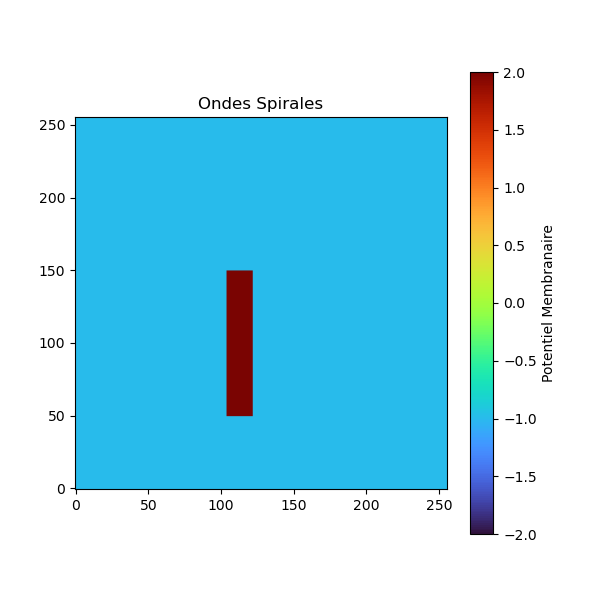
\includegraphics[width=\linewidth]{Figures/Potentiel.png}
\caption{État initial : domaine excité (rouge) et domaine au repos (bleu).}
\end{figure}
\end{columns}
\end{frame}

\begin{frame}
\frametitle{Simulation numérique}
\framesubtitle{Apparition d'une onde spirale}
\begin{columns}
\column{0.45\textwidth}
\begin{itemize}
  \item La pointe de la spirale tourne autour d’une zone centrale qui ne s’excite jamais.
  \item Le front d’onde parcourt le domaine périodiquement ; chaque point du tissu est excité une fois par rotation.
  \item Cette structure auto‑entretenue correspond aux réentrées fonctionnelles observées dans le myocarde.
\end{itemize}
\column{0.55\textwidth}
\centering
\begin{figure}
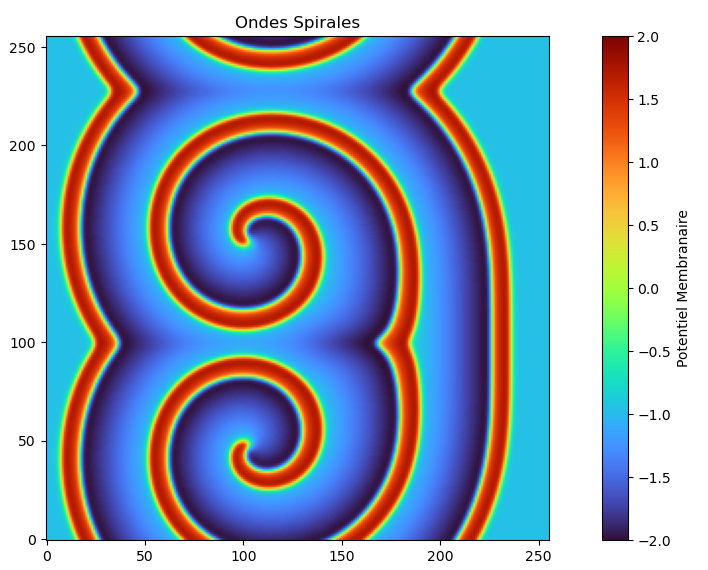
\includegraphics[width=\linewidth]{Figures/Spiral.png}
\caption{Instant de la simulation montrant l’onde spirale (échelle de couleurs : potentiel $v$).}
\end{figure}
\end{columns}
\end{frame}
\section{Interprétation et exploitation}

\begin{frame}
\frametitle{Interprétation et exploitation}
\framesubtitle{Apport du modèle FHN}
\begin{itemize}
  \item Sa simplicité permet d'isoler les mécanismes essentiels de l'excitabilité.
  \item Il permet la simulation de phénomènes complexes comme les ondes spirales.
  \item Ces ondes spirales sont responsables d'arythmies.
\end{itemize}
\end{frame}

\begin{frame}
\frametitle{Interprétation et exploitation}
\framesubtitle{Application à la défibrillation cardiaque}
\begin{figure}
\caption{Dissolution du noyau d'une onde spirale}
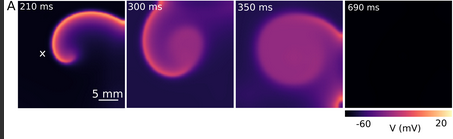
\includegraphics[width = \linewidth]{Figures/Breakup.png}
\source{(2023) Dissolution of spiral wave’s core using
cardiac optogenetics. PLoS Comput Biol 19(12):
e1011660}
\end{figure}
\end{frame}

\begin{frame}
\begin{center}
\textbf{Merci de votre attention}
\end{center}
\end{frame}
\section{Annexe}

\begin{frame}[fragile]
\frametitle{Annexe 1 : Génération des isoclines et trajectoires}
\begin{mintedbox}[fontsize=\tiny]{python}
import numpy as np
import matplotlib.pyplot as plt

a = 0.9
b = 0.5
epsilon = 0.08
Ip = 1
T = 200
dt = 0.01
t = np.arange(0, T, dt)

v = np.zeros(len(t))
w = np.zeros(len(t))
v[0] = 0
w[0] = 0

for i in range(len(t) - 1):
    dv = v[i] - v[i]**3 / 3 - w[i] + Ip
    dw = epsilon * (v[i] + a - b * w[i])
    v[i + 1] = v[i] + dt * dv
    w[i + 1] = w[i] + dt * dw

v_plot = np.linspace(-2.5, 2.5, 500)
w_null2 = (v_plot + a) / b
w_null_v = v_plot - v_plot**3 / 3 + Ip

plt.figure(figsize=(5, 5))
plt.plot(v_plot, w_null_v, label="dv/dt = 0")
plt.plot(v_plot, w_null2, label="dw/dt = 0")
plt.plot(v, w, alpha=0.6, label="Trajectoire")
plt.xlabel("Potentiel membranaire v")
plt.ylabel("Variable de récupération w")
plt.ylim(-1,3)
plt.legend()
plt.grid()
plt.show()
\end{mintedbox}
\end{frame}

\begin{frame}[fragile]
\frametitle{Annexe 2 : Tracé temporel}
\begin{mintedbox}[fontsize=\tiny]{python}
...
for i in range(len(t) - 1):
    dv = v[i] - v[i]**3 / 3 - w[i] + Ip
    dw = epsilon * (v[i] + a - b * w[i])
    v[i + 1] = v[i] + dt * dv
    w[i + 1] = w[i] + dt * dw
    
plt.figure(figsize=(10, 4))
plt.plot(t, v, label="v(t) : potentiel")
plt.plot(t, w, label="w(t) : récupération")
plt.xlabel("Temps")
plt.ylabel("Variables")
plt.legend()
plt.title("Modèle de FitzHugh–Nagumo")
plt.grid()
plt.show()

\end{mintedbox}
\end{frame}

\begin{frame}[fragile]
\frametitle{Annexe 3 : Comparaison avec modèle linéaire}
\begin{mintedbox}[fontsize=\tiny]{python}
T = 150
dt = 0.01
t = np.arange(0, T, dt)
v = np.zeros(len(t))
w = np.zeros(len(t))
v_lin = np.zeros(len(t))
w_lin = np.zeros(len(t))
v[0] = 0
w[0] = 0
v_lin[0] = 0
w_lin[0] = 0

for i in range(len(t) - 1):
    dv = v[i] - v[i]**3/3 - w[i] + Ip
    dw = epsilon * (v[i] + a - b * w[i])
    v[i+1] = v[i] + dt * dv
    w[i+1] = w[i] + dt * dw
    if v_lin[i] < va: dv_lin = c * v_lin[i] - d - w_lin[i] + Ip
    elif v_lin[i] > vb: dv_lin = c * v_lin[i] + d - w_lin[i] + Ip
    else: dv_lin = (2/3) * v_lin[i] - w_lin[i] + Ip
    dw_lin = epsilon * (v_lin[i] + a - b * w_lin[i])
    v_lin[i+1] = v_lin[i] + dt * dv_lin
    w_lin[i+1] = w_lin[i] + dt * dw_lin

v_plot = np.linspace(-3, 3, 500)
plt.figure(figsize=(6, 6))
plt.plot(t,v, label = "cubique")
plt.plot(t,v_lin, label = "linéaire par morceaux")
plt.xlabel('t')
plt.ylabel('v')
plt.grid()
plt.legend( )
plt.title('Allure de la réponse')
plt.show()
\end{mintedbox}
\end{frame}

\begin{frame}[fragile]
\frametitle{Annexe 4-1: Approximation du Laplacien}
\begin{itemize}

\item{Approximation du laplacien par différences finies centrées à cinq
points}
  \[
  \nabla^2 v_{i,j} \approx \frac{v_{i+1,j} + v_{i-1,j} + v_{i,j+1} + v_{i,j-1} - 4v_{i,j}}{\Delta x^2}.
  \]
\end{itemize}
\begin{mintedbox}[fontsize=\small]{python}
def laplacian(Z):
    return (
        np.roll(Z, 1, axis=0) +
        np.roll(Z, -1, axis=0) +
        np.roll(Z, 1, axis=1) +
        np.roll(Z, -1, axis=1) -
        4 * Z
    ) / dx**2
\end{mintedbox}
\end{frame}

\begin{frame}[fragile]
\frametitle{Annexe 4-2: Initialisation du Tissu et des variables}

\begin{mintedbox}[fontsize=\footnotesize]{python}
import numpy as np
import matplotlib.pyplot as plt

Nx, Ny = 256, 256
dx = 1.0
dt = 0.01
steps = 15000
plot_every = 40

D = 1.0
a = 0.8
b = 0.3
epsilon = 0.08
epsilon_Field = epsilon * (1 + 0.0 * np.random.randn(Nx, Ny))
v = -1.0 * np.ones((Nx, Ny))  
w = -0.5 * np.ones((Nx, Ny))  

v[50:150,Ny//2-4-20:Ny//2+4-10] = 2.0
w[50:150,Ny//2-4-30:Ny//2+4-10] = 0.0
\end{mintedbox}
\end{frame}

\begin{frame}[fragile]
\frametitle{Annexe 4-3: Simulation et visualisation}
\begin{mintedbox}[fontsize=\footnotesize]{python}
plt.figure(figsize=(6, 6))
img = plt.imshow(v, cmap="turbo", origin="lower", animated=True, vmin=-2, vmax=2)
plt.colorbar(label="Potentiel Membranaire")
plt.title("Ondes Spirales")

for n in range(steps):
    Lv = laplacian(v)                     
    dv = v - (v**3) / 3 - w + D * Lv      
    dw = epsilon_Field * (v + a - b * w) 
    v += dt * dv
    w += dt * dw
    if n % plot_every == 1:
        img.set_data(v)          
        plt.draw()
        plt.pause(0.0005)

plt.show()
\end{mintedbox}
\end{frame}
\end{document}
